% MRANet architecture diagram (Figure 1)
% Compile: pdflatex fig1_architecture.tex
\documentclass[tikz,border=5pt]{standalone}
\usepackage{tikz}
\usetikzlibrary{positioning, arrows.meta, fit, calc}

\begin{document}
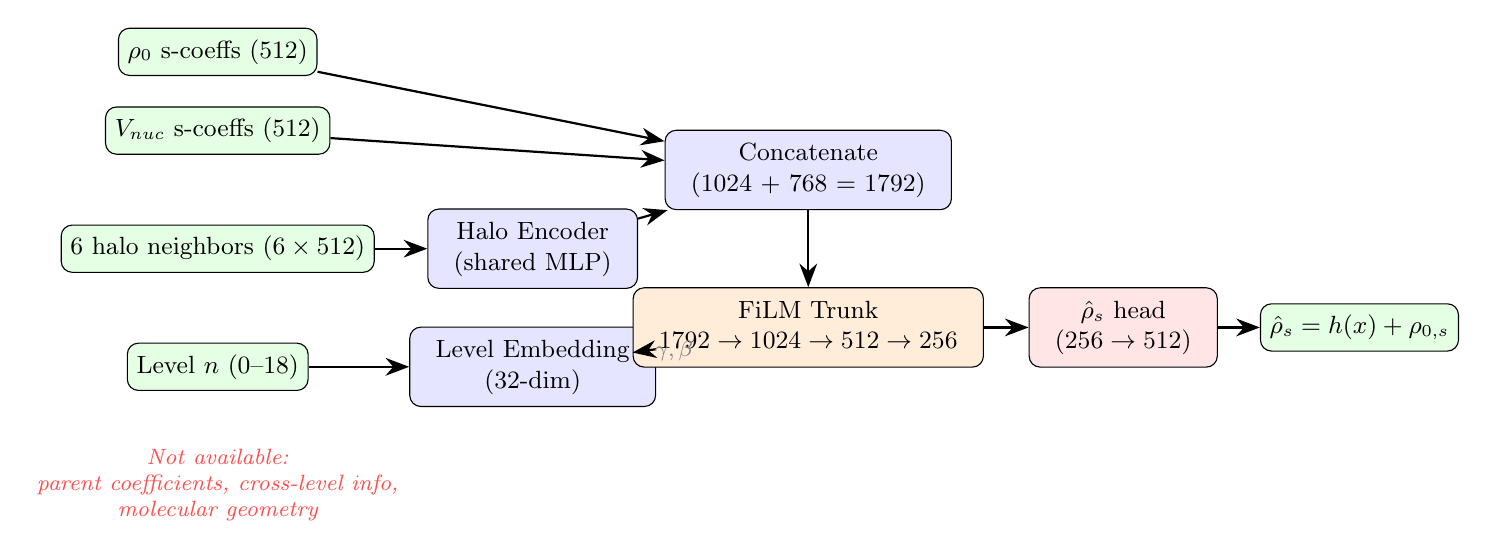
\begin{tikzpicture}[
    block/.style={draw, rounded corners, minimum height=0.8cm, minimum width=2cm, fill=blue!10, font=\small},
    data/.style={draw, rounded corners, minimum height=0.6cm, fill=green!10, font=\small},
    arrow/.style={-{Stealth[length=3mm]}, thick},
    note/.style={font=\footnotesize\itshape, text=gray},
]

% Input features
\node[data] (rho0) at (0, 3) {$\rho_0$ s-coeffs (512)};
\node[data] (vnuc) at (0, 2) {$V_\text{nuc}$ s-coeffs (512)};
\node[data] (halo) at (0, 0.5) {6 halo neighbors ($6\times512$)};
\node[data] (level) at (0, -1) {Level $n$ (0--18)};

% Encoders
\node[block] (halo_enc) at (4, 0.5) {\begin{tabular}{c}Halo Encoder\\(shared MLP)\end{tabular}};
\node[block] (level_emb) at (4, -1) {\begin{tabular}{c}Level Embedding\\(32-dim)\end{tabular}};

% Concatenation
\node[block, minimum width=3cm] (concat) at (7.5, 1.5) {\begin{tabular}{c}Concatenate\\(1024 + 768 = 1792)\end{tabular}};

% FiLM trunk
\node[block, fill=orange!15, minimum width=3cm] (trunk) at (7.5, -0.5) {\begin{tabular}{c}FiLM Trunk\\$1792 \to 1024 \to 512 \to 256$\end{tabular}};

% Output
\node[block, fill=red!10] (head) at (11.5, -0.5) {\begin{tabular}{c}$\hat{\rho}_s$ head\\($256 \to 512$)\end{tabular}};
\node[data] (output) at (14.5, -0.5) {$\hat{\rho}_s = h(x) + \rho_{0,s}$};

% Arrows
\draw[arrow] (rho0) -- (concat);
\draw[arrow] (vnuc) -- (concat);
\draw[arrow] (halo) -- (halo_enc);
\draw[arrow] (halo_enc) -- (concat);
\draw[arrow] (concat) -- (trunk);
\draw[arrow] (level_emb) -- node[right, note] {$\gamma, \beta$} (trunk);
\draw[arrow] (level) -- (level_emb);
\draw[arrow] (trunk) -- (head);
\draw[arrow] (head) -- (output);

% Annotation: what the model does NOT see
\node[note, text=red!70, align=center] at (0, -2.5) {Not available:\\parent coefficients, cross-level info,\\molecular geometry};

\end{tikzpicture}
\end{document}
